\documentclass{standalone}
\usepackage{tikz}
\usetikzlibrary{patterns, positioning}
\usepackage[sfdefault]{ClearSans} %% option 'sfdefault' activates Clear Sans as the default text font
\usepackage[T1]{fontenc}

\begin{document}
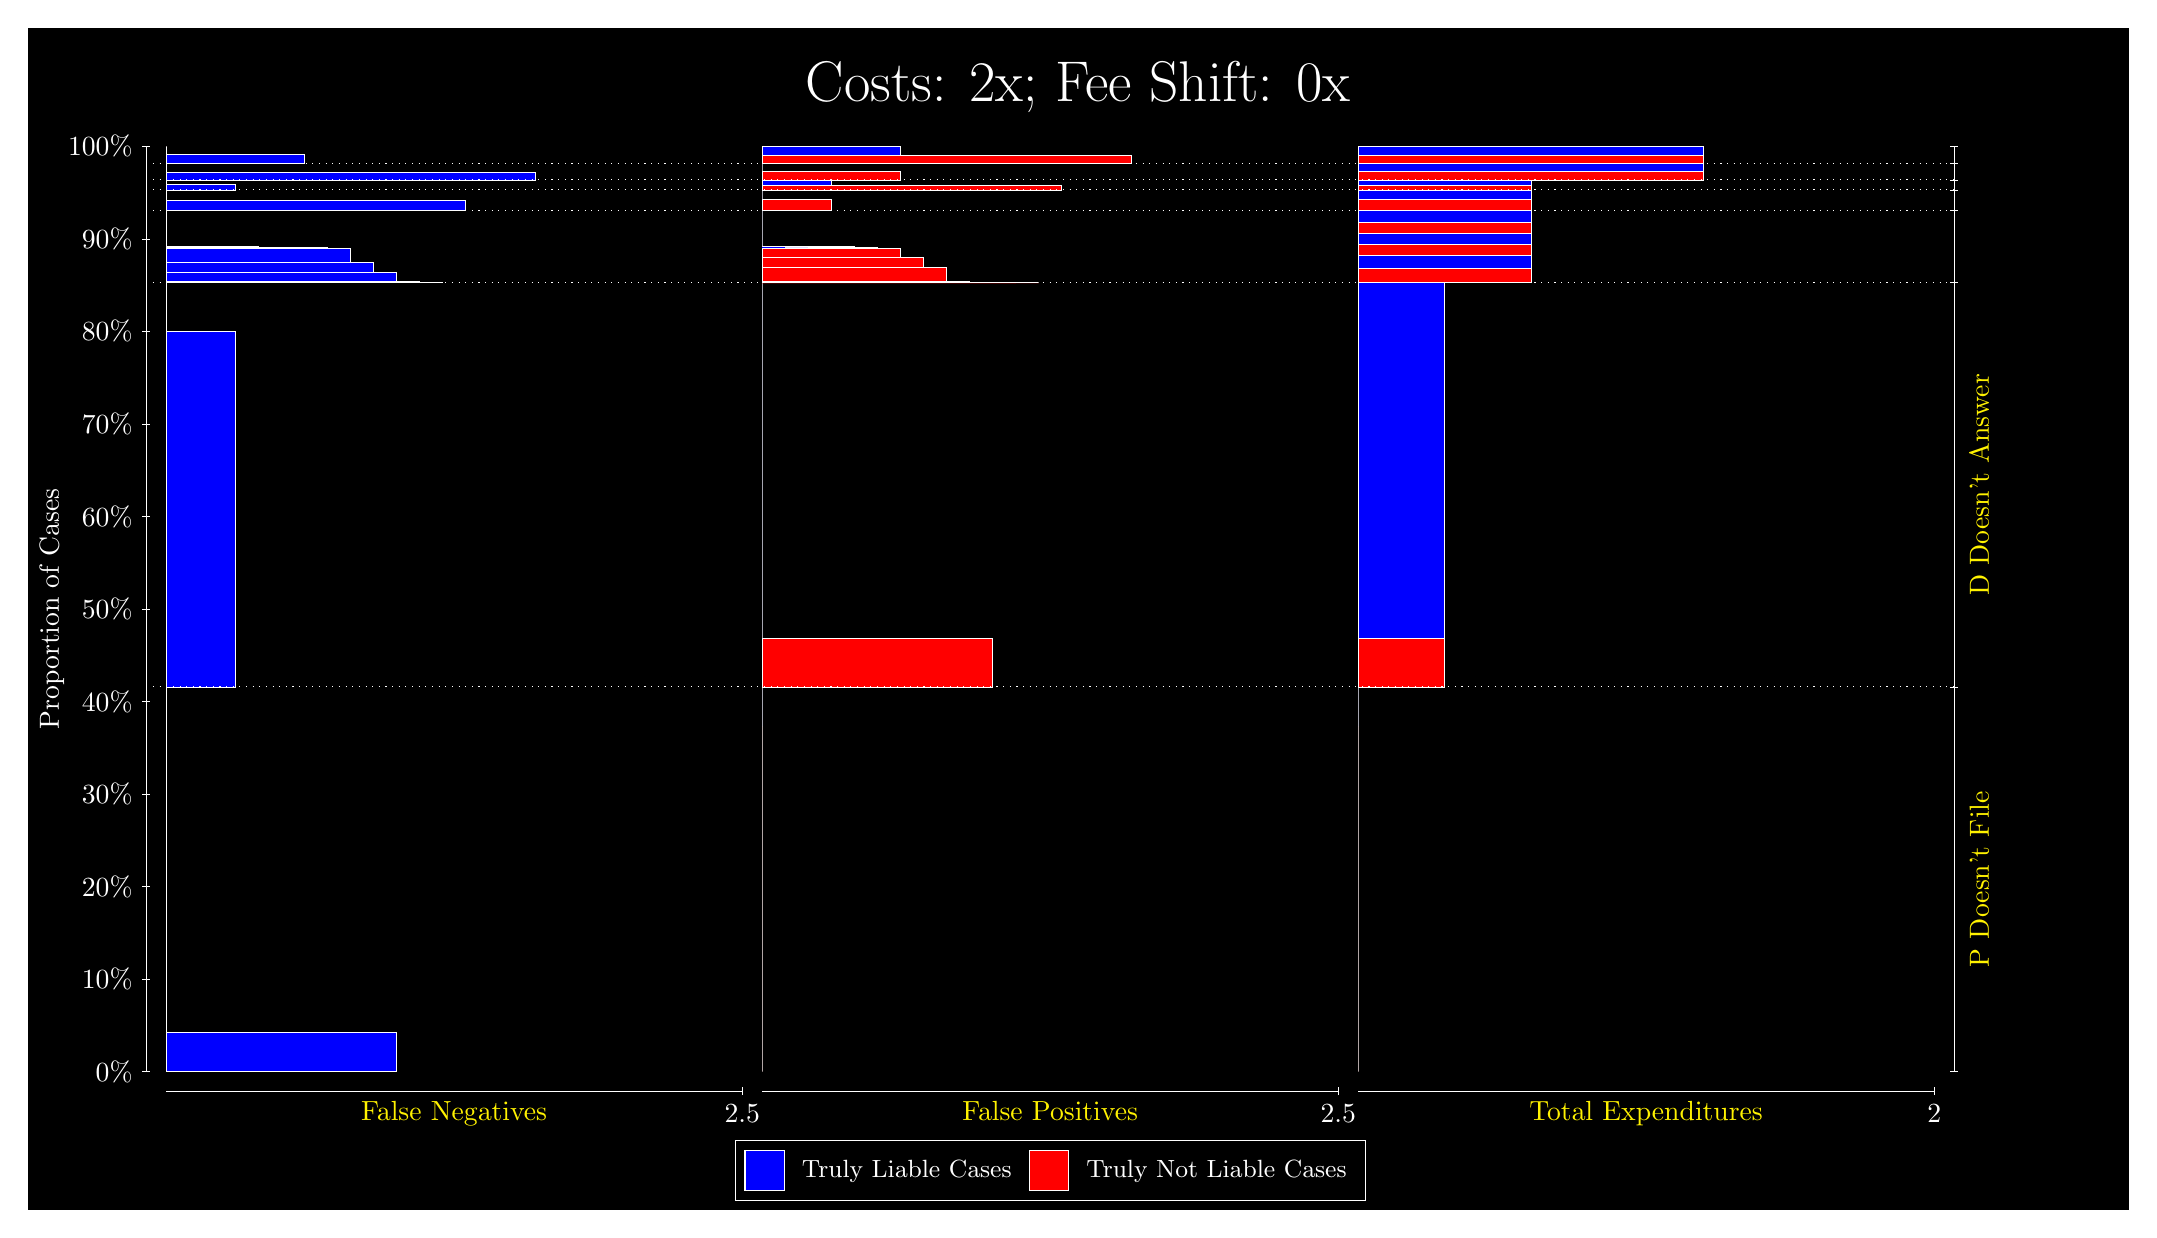
\begin{tikzpicture}
\draw[fill=black] (0,0) rectangle (26.667,15);
\draw[text=white] (0,13.5) rectangle (26.667,15) node[midway] {\huge Costs: 2x; Fee Shift: 0x};
\draw[white, very thin] (1.5,1.75) -- (1.5,13.5);
\node[rotate=90, text=white, anchor=center] at (0.3, 7.625) {Proportion of Cases};
\draw[white, very thin] (1.45,1.75) -- (1.55,1.75);
\node[text=white, anchor=east] at (1.45, 1.75) {0\%};
\draw[white, very thin] (1.45,2.925) -- (1.55,2.925);
\node[text=white, anchor=east] at (1.45, 2.925) {10\%};
\draw[white, very thin] (1.45,4.1) -- (1.55,4.1);
\node[text=white, anchor=east] at (1.45, 4.1) {20\%};
\draw[white, very thin] (1.45,5.275) -- (1.55,5.275);
\node[text=white, anchor=east] at (1.45, 5.275) {30\%};
\draw[white, very thin] (1.45,6.45) -- (1.55,6.45);
\node[text=white, anchor=east] at (1.45, 6.45) {40\%};
\draw[white, very thin] (1.45,7.625) -- (1.55,7.625);
\node[text=white, anchor=east] at (1.45, 7.625) {50\%};
\draw[white, very thin] (1.45,8.8) -- (1.55,8.8);
\node[text=white, anchor=east] at (1.45, 8.8) {60\%};
\draw[white, very thin] (1.45,9.975) -- (1.55,9.975);
\node[text=white, anchor=east] at (1.45, 9.975) {70\%};
\draw[white, very thin] (1.45,11.15) -- (1.55,11.15);
\node[text=white, anchor=east] at (1.45, 11.15) {80\%};
\draw[white, very thin] (1.45,12.325) -- (1.55,12.325);
\node[text=white, anchor=east] at (1.45, 12.325) {90\%};
\draw[white, very thin] (1.45,13.5) -- (1.55,13.5);
\node[text=white, anchor=east] at (1.45, 13.5) {100\%};

\draw[white, very thin] (24.457,1.75) -- (24.457,13.5);
\draw[white, very thin] (24.407,1.75) -- (24.507,1.75);
\node[anchor=west] at (24.407, 1.75) {};
\draw[white, very thin] (24.407,6.6358) -- (24.507,6.6358);
\node[anchor=west] at (24.407, 6.6358) {};
\draw[white, very thin] (24.407,11.768) -- (24.507,11.768);
\node[anchor=west] at (24.407, 11.768) {};
\draw[white, very thin] (24.407,12.683) -- (24.507,12.683);
\node[anchor=west] at (24.407, 12.683) {};
\draw[white, very thin] (24.407,12.948) -- (24.507,12.948);
\node[anchor=west] at (24.407, 12.948) {};
\draw[white, very thin] (24.407,13.073) -- (24.507,13.073);
\node[anchor=west] at (24.407, 13.073) {};
\draw[white, very thin] (24.407,13.285) -- (24.507,13.285);
\node[anchor=west] at (24.407, 13.285) {};
\draw[white, very thin] (24.407,13.5) -- (24.507,13.5);
\node[anchor=west] at (24.407, 13.5) {};

\draw[white, very thin, fill=blue] (1.75,1.75) rectangle (4.6775,2.2488);
\draw[white, very thin, fill=red] (1.75,2.2488) rectangle (1.75,6.6358);
\draw[white, very thin, fill=blue] (1.75,6.6358) rectangle (2.6283,11.148);
\draw[white, very thin, fill=red] (1.75,11.148) rectangle (1.75,11.768);
\draw[white, very thin, fill=blue] (1.75,11.768) rectangle (5.2631,11.772);
\draw[white, very thin, fill=blue] (1.75,11.772) rectangle (4.9703,11.782);
\draw[white, very thin, fill=blue] (1.75,11.782) rectangle (4.6775,11.901);
\draw[white, very thin, fill=blue] (1.75,11.901) rectangle (4.3848,11.902);
\draw[white, very thin, fill=blue] (1.75,11.902) rectangle (4.3848,12.031);
\draw[white, very thin, fill=blue] (1.75,12.031) rectangle (4.092,12.203);
\draw[white, very thin, fill=blue] (1.75,12.203) rectangle (3.7993,12.22);
\draw[white, very thin, fill=blue] (1.75,12.22) rectangle (3.5065,12.224);
\draw[white, very thin, fill=blue] (1.75,12.224) rectangle (3.2138,12.224);
\draw[white, very thin, fill=blue] (1.75,12.224) rectangle (2.921,12.225);
\draw[white, very thin, fill=red] (1.75,12.225) rectangle (1.75,12.683);
\draw[white, very thin, fill=blue] (1.75,12.683) rectangle (5.5558,12.809);
\draw[white, very thin, fill=red] (1.75,12.809) rectangle (1.75,12.948);
\draw[white, very thin, fill=blue] (1.75,12.948) rectangle (2.6283,13.014);
\draw[white, very thin, fill=red] (1.75,13.014) rectangle (1.75,13.073);
\draw[white, very thin, fill=blue] (1.75,13.073) rectangle (6.4341,13.169);
\draw[white, very thin, fill=red] (1.75,13.169) rectangle (1.75,13.285);
\draw[white, very thin, fill=blue] (1.75,13.285) rectangle (3.5065,13.403);
\draw[white, very thin, fill=red] (1.75,13.403) rectangle (1.75,13.5);
\draw[white, very thin, fill=red] (9.3189,1.75) rectangle (9.3189,6.137);
\draw[white, very thin, fill=blue] (9.3189,6.137) rectangle (9.3189,6.6358);
\draw[white, very thin, fill=red] (9.3189,6.6358) rectangle (12.246,7.2555);
\draw[white, very thin, fill=blue] (9.3189,7.2555) rectangle (9.3189,11.768);
\draw[white, very thin, fill=red] (9.3189,11.768) rectangle (12.832,11.768);
\draw[white, very thin, fill=red] (9.3189,11.768) rectangle (12.539,11.768);
\draw[white, very thin, fill=red] (9.3189,11.768) rectangle (12.246,11.773);
\draw[white, very thin, fill=red] (9.3189,11.773) rectangle (11.954,11.79);
\draw[white, very thin, fill=red] (9.3189,11.79) rectangle (11.661,11.962);
\draw[white, very thin, fill=red] (9.3189,11.962) rectangle (11.368,12.092);
\draw[white, very thin, fill=red] (9.3189,12.092) rectangle (11.075,12.211);
\draw[white, very thin, fill=red] (9.3189,12.211) rectangle (10.783,12.22);
\draw[white, very thin, fill=red] (9.3189,12.22) rectangle (10.49,12.226);
\draw[white, very thin, fill=blue] (9.3189,12.226) rectangle (9.9044,12.226);
\draw[white, very thin, fill=blue] (9.3189,12.226) rectangle (9.6116,12.227);
\draw[white, very thin, fill=blue] (9.3189,12.227) rectangle (9.3189,12.683);
\draw[white, very thin, fill=red] (9.3189,12.683) rectangle (10.197,12.822);
\draw[white, very thin, fill=blue] (9.3189,12.822) rectangle (9.3189,12.948);
\draw[white, very thin, fill=red] (9.3189,12.948) rectangle (13.125,13.007);
\draw[white, very thin, fill=blue] (9.3189,13.007) rectangle (10.197,13.073);
\draw[white, very thin, fill=red] (9.3189,13.073) rectangle (11.075,13.188);
\draw[white, very thin, fill=blue] (9.3189,13.188) rectangle (9.3189,13.285);
\draw[white, very thin, fill=red] (9.3189,13.285) rectangle (14.003,13.382);
\draw[white, very thin, fill=blue] (9.3189,13.382) rectangle (11.075,13.5);
\draw[white, very thin, fill=red] (16.888,1.75) rectangle (16.888,6.137);
\draw[white, very thin, fill=blue] (16.888,6.137) rectangle (16.888,6.6358);
\draw[white, very thin, fill=red] (16.888,6.6358) rectangle (17.986,7.2555);
\draw[white, very thin, fill=blue] (16.888,7.2555) rectangle (17.986,11.768);
\draw[white, very thin, fill=red] (16.888,11.768) rectangle (19.083,11.945);
\draw[white, very thin, fill=blue] (16.888,11.945) rectangle (19.083,12.122);
\draw[white, very thin, fill=red] (16.888,12.122) rectangle (19.083,12.257);
\draw[white, very thin, fill=blue] (16.888,12.257) rectangle (19.083,12.391);
\draw[white, very thin, fill=red] (16.888,12.391) rectangle (19.083,12.537);
\draw[white, very thin, fill=blue] (16.888,12.537) rectangle (19.083,12.683);
\draw[white, very thin, fill=red] (16.888,12.683) rectangle (19.083,12.822);
\draw[white, very thin, fill=blue] (16.888,12.822) rectangle (19.083,12.948);
\draw[white, very thin, fill=red] (16.888,12.948) rectangle (19.083,13.007);
\draw[white, very thin, fill=blue] (16.888,13.007) rectangle (19.083,13.073);
\draw[white, very thin, fill=red] (16.888,13.073) rectangle (21.279,13.188);
\draw[white, very thin, fill=blue] (16.888,13.188) rectangle (21.279,13.285);
\draw[white, very thin, fill=red] (16.888,13.285) rectangle (21.279,13.382);
\draw[white, very thin, fill=blue] (16.888,13.382) rectangle (21.279,13.5);
\draw[white, dotted] (1.5,6.6358) -- (24.457,6.6358);
\draw[white, dotted] (1.5,11.768) -- (24.457,11.768);
\draw[white, dotted] (1.5,12.683) -- (24.457,12.683);
\draw[white, dotted] (1.5,12.948) -- (24.457,12.948);
\draw[white, dotted] (1.5,13.073) -- (24.457,13.073);
\draw[white, dotted] (1.5,13.285) -- (24.457,13.285);
\draw[white, very thin] (1.75,1.5) -- (9.0689,1.5);
\node[text=yellow, anchor=north] at (5.4094, 1.5) {False Negatives};
\draw[white, very thin] (9.0689,1.45) -- (9.0689,1.55);
\node[text=white, anchor=north] at (9.0689, 1.45) {2.5};

\draw[white, very thin] (9.3189,1.5) -- (16.638,1.5);
\node[text=yellow, anchor=north] at (12.978, 1.5) {False Positives};
\draw[white, very thin] (16.638,1.45) -- (16.638,1.55);
\node[text=white, anchor=north] at (16.638, 1.45) {2.5};

\draw[white, very thin] (16.888,1.5) -- (24.207,1.5);
\node[text=yellow, anchor=north] at (20.547, 1.5) {Total Expenditures};
\draw[white, very thin] (24.207,1.45) -- (24.207,1.55);
\node[text=white, anchor=north] at (24.207, 1.45) {2};

\node[text=yellow, centered, rotate=90] at (24.777, 4.1929) {P Doesn't File};
\node[text=yellow, centered, rotate=90] at (24.777, 9.2018) {D Doesn't Answer};






\draw (12.978300999999998,1.5) node[draw=none] (baseCoordinate) {};
\begin{scope}[align=center]
        \matrix[scale=0.5, draw=white, below=0.5cm of baseCoordinate, nodes={draw}, column sep=0.1cm]{
            \node[rectangle, draw, minimum width=0.5cm, minimum height=0.5cm, fill=blue] {}; &
            \node[draw=none, font=\small, text=white] (B) {Truly Liable Cases}; &
            \node[rectangle, draw, minimum width=0.5cm, minimum height=0.5cm, fill=red] {}; &
            \node[draw=none, font=\small, text=white] (B) {Truly Not Liable Cases}; \\
            };
\end{scope}

\end{tikzpicture}
\end{document}